\documentclass[../main-00.tex]{subfiles}
\begin{document}
\chapter{Use Cases}
\label{ch:use}
\section{Introduction}

In this chapter we describe some of the known use-cases for DUNE computing.  We start with the protoDUNE cases, using lessons learned from the 2018 run to understand the performance of future far detector modules. 


%%%%%%%%%%%%%%%%%%%%%%%%%%%%%%%%


\section{ProtoDUNEdata: raw data acquisition, cataloging and storage}\label{sec:use:pdii-daq}



\subsection{ProtoDUNE Data: DAQ to Raw Data store}
The \dword{daq} and \dword{cisc} systems are expected to provide in close to real time:

\begin{itemize}
    \item Raw data from the \dword{tpc} and \dword{pd} detectors. 
    \item Information on run and trigger configuration
    \item Beam information
    \item Information on detector conditions. For example, granular information on the \dword{hv} is needed to study and compensate for \dword{hv} fluctuations. 
    \item Low level calibration constants such as gains that do not need extensive offline processing
    
\end{itemize}


The raw data are written to disk locally and then copied to the archive site (FNAL). Once the data are confirmed to be on tape, the local copy may be deleted.

A second copy of the raw data will be stored in a different archive. 

The run and trigger information, beamline  data, conditions and calibration constants are made available through separate data paths and stored in appropriate databases. In ProtoDUNE Run I, some of this information was transferred manually and stored in the \dword{sam} catalog.  DUNE document 22983 \cite{bib:docdb22983} describes the metadata strategy for ProtoDUNE II and DUNE. 


\section{ProtoDUNE data: reconstruction - hits}\label{sec:use:pdii}

Figure \ref{fig:ch:use:pdii} shows the data flow for regular reconstruction.  There are in principle, multiple stages in reconstruction that are well suited to different computer architectures.  We expect the full \dword{fd} data processing to follow a similar path. 

\subsection{Raw data to reconstructed hits}

This step takes the raw waveforms, applies  basic channel-to-channel calibrations, removes noise and stuck bits and performs 2D deconvolution.   This processing step operates on large 2-D data arrays and may be suitable for different architectures than conventional pattern recognition. It is anticipated that this step will not need to be done frequently. 

The input data at this point are quite uniform, effectively bit streams from \dword{tpc} and \dword{pd} channels.  There are correlations between channels in \dword{tpc} data which require concurrent processing of multiple channels.  Segmentation at the level of a readout plane within an \dword{apa}  or \dword{lem} is desirable.  An uncompressed \dword{apa} plane is of order 10 MB of 12-bit words. 

The outputs are gaussian fits to the pulses 



\subsection{Hits to Calibration}

In this step, the processed hits from calibration samples (subsets of the full data, sometimes with special conditions) are run through specialized pattern recognition and used to derive high quality calibration constants which are stored in the conditions database for future use.   This step will likely be done many times, especially at experiment start.

\subsection{Hits to reconstructed interactions }
In this step, the improved calibration constants and raw hits are input to the full  pattern recognition and reconstructed interactions are output. Data quality can be monitored as part of this processing and stored. 

Here a wide range of algorithms may be used.  

\subsection{Interactions to Analysis}
The interaction data, which is in the output format supplied by the full reconstruction is reduced and reconfigured into analysis formats for use by users. 

In the long run this processing will be done as coherent production steps but is currently being done by small groups.

A typical \dword{pdsp} data or simulation sample reads in  of around 1,000-10,000 4-8 GB reconstructed files and produces much smaller tuple outputs for analysis.  These jobs stream using \dword{xrootd} and are IO bound. Preliminary monitoring studies indicate that average input rates of 30 MB/sec per process can be achieved within a single site, with aggregate rates of several GB/sec across multiple processes. We are currently mining data access records to measure rates and reliability as a function of source and sink. 

\subsection{Analysis}
Analysis samples should be small and useful.  Analysis codes should not need to read from the central databases but may access small local replicas. 


\begin{dunefigure}
[Data flow diagram for standard ProtoDUNE reconstruction]
{fig:ch:use:pdii}
{Data flow diagram for standard ProtoDUNE data reconstruction.}
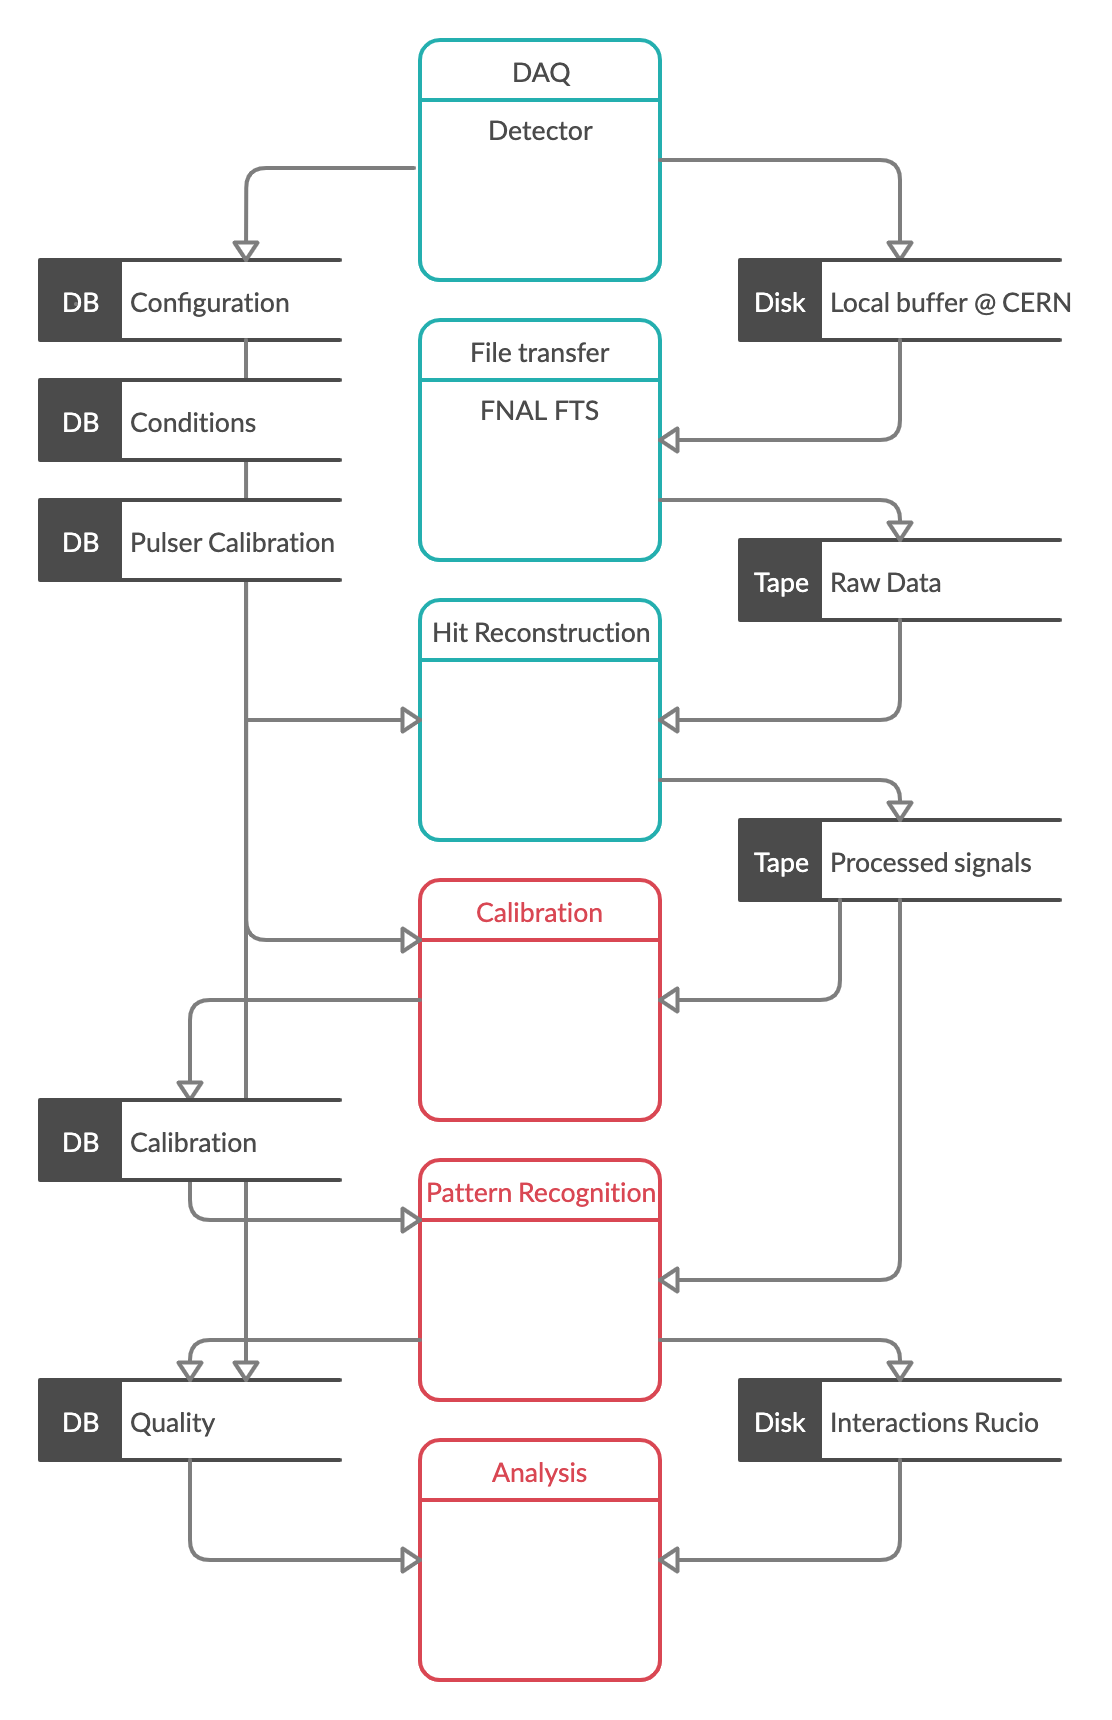
\includegraphics[width=0.8\textwidth]{graphics/IntroFigures/DataProcessingPDv1.png}
\end{dunefigure}
\pagebreak


%\section{Data reduction at FNAL before writing it out?}

%\section{Fast processing for data monitoring} 

\section{Normal  and SNB Far Detector: acquisition and reconstruction}
\label{sec:use:fdbeam}  %% fix label according to section

\begin{dunefigure}
[Data aggregation diagram for FD]
{fig:ch:use:fdagg}
{Data aggregation cases for the far detector. The top case shows information for normal beam or calibration readouts. A single file of $\sim 10$GB size contains several complete trigger readouts with their boundaries designated by the dashed lines.  TPC APA's, Photon Detector (PD),  trigger primitives and a trigger  are recorded for each trigger readout.  In addition, a manifest which describes the relations between the data is stored, either in the file or in metadata.  The bottom case is a supernova readout, in which thousands of 5-10 ms time slices must be read out over 100 sec.  The solid lines denote file boundaries. How data ordered, by geographical position or by team is not specified.}
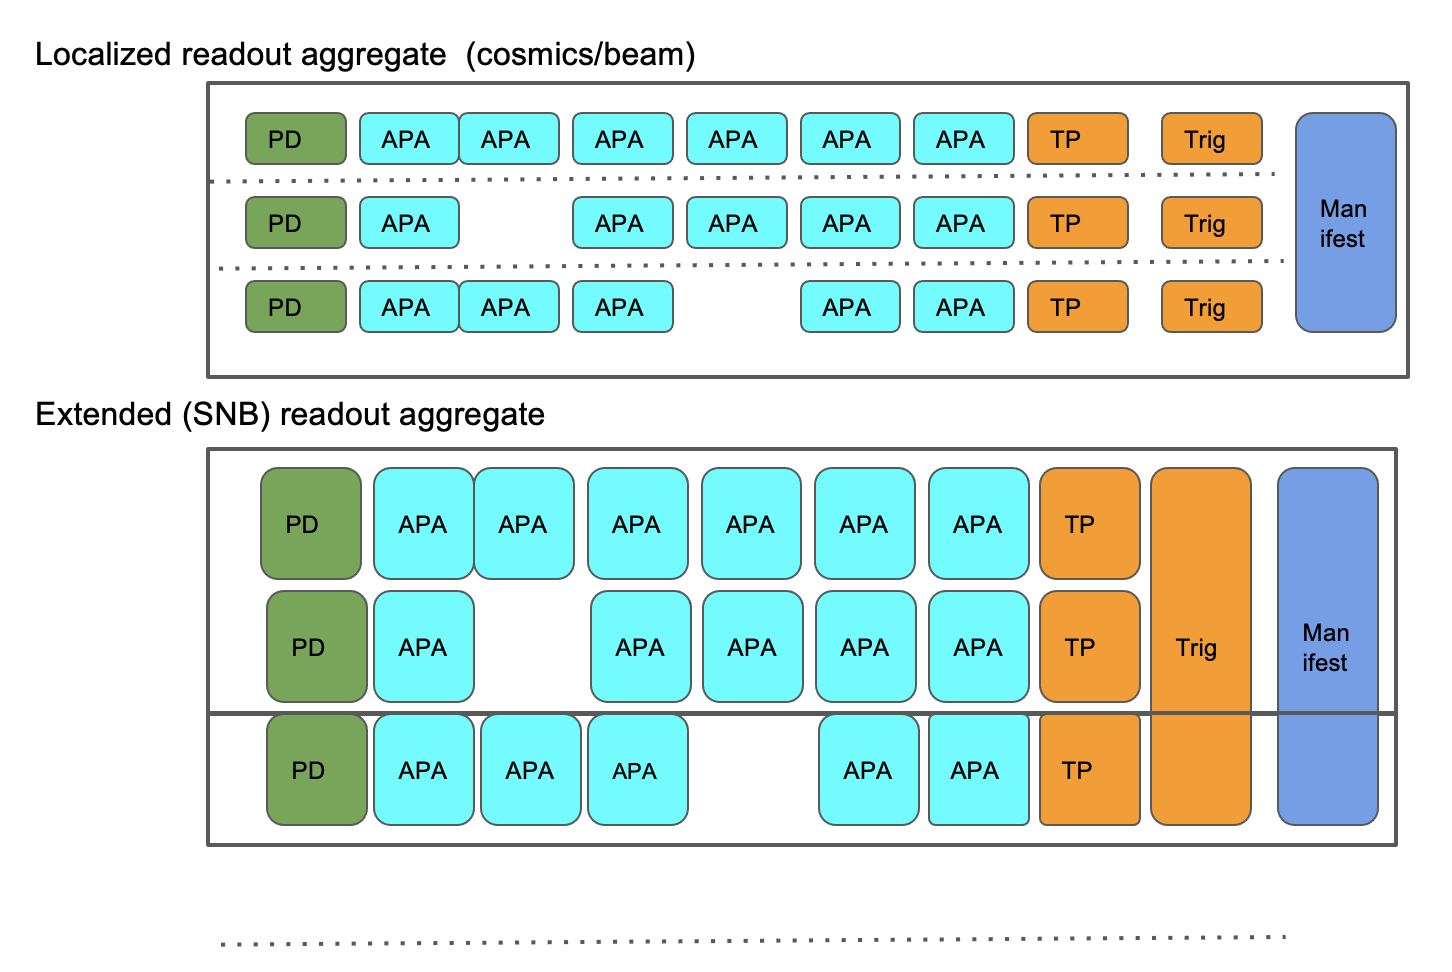
\includegraphics[width=0.8\textwidth]{graphics/IntroFigures/DataAggregation.png}
\end{dunefigure}
%\pagebreak

\subsection{ProtoDUNE simulation}

\fixme{need some text here on simulation}
 
\section{DUNE Beam Data: Beam data acquisition and reconstruction \hideme{ Mathew Muether/Tom Junk}}
\label{sec:use:ndbeam}  %% fix label according to section

\section{DUNE Simulation}  \fixme{Mathews' diagram} 

Simulation shares a reconstruction path with real data but begins differently.

\subsection{Beam simulation}\label{sec:use:beamsim}
Tbe neutrino beam is simulated using g4lbnf\cite{g4lbnf} a geant4 based simulation of the beamline components.  Intermediate interactions are stored so that cross section reweighting can be applied.  The beam simulation is generally done separately and beam files are stored and used when needed. 

%\subsection{Cosmic simulation?}

\todo{how big are events?  what are memory/CPU requirements}

The far and near detectors subtend very different solid angles so one has to simulate a very large number of events or use reweighting techniques to properly cover both. 

%\subsection{Cosmic simulation?}

\subsection{Interaction simulation}\label{sec:use:intmodel}
Next an event generator is used to simulate the primary interaction.  This step requires a reasonably accurate geometry for the detectors to account for different target materials and, for the near detector, different locations. Simulation parameters and reasonably detailed event information need to be stored to allow for subsequent reweighting.  

\subsection{Particle tracing}\label{sec:use:tracing}
The geant4 simulation package is then used to simulate the energy deposited by final state particles as they pass through the detector.  Both ionization and scintillation signatures need to be recorded.  

\subsection{Detector response simulation}\label{sec:use:detsim}
Once geant4 has simulated the energy deposit, detailed simulation of charge and light collection and electronics response can be done.  

\subsection{Overlay}\label{sec:use:overlay}
It is often useful to overlay real data on simulation to fully account for cosmic ray and upstream neutrino interactions. This adds complexity as the real data must be delivered to simulation jobs and be properly matched to the running conditions for the simulation.  The "electronics" signals from real data and simulation need to be mixed and stored.  The \dword{microboone} experiment has adapted \dword{larsoft} to do this and we plan to build on that experience. 

\todo{Discussion of overlay experience from MicroBooNE - Kirby}

\subsection{Reconstruction} \label{sec:use:mcreco}
Reconstruction and analysis can then be performed using the same methods as in section \ref{sec:use:pdii}.  Due to the large amount of interaction and intermediate step information kept for studies, simulated events are often several times the size of real data.  A significant question, given the size of events, is whether it may be more efficient to regenerate than to store all the information needed for reweighting. 


\todo{add a table showing \# of events, CPU and memory footprint for each step}









\section{Oscillation analysis} Chris Backhouse?  Chris Marshall? 
\label{sec:use:osc}

\section{Supernova data: acquisition and fast reconstruction}
\label{sec:use:supernova}  %% fix label according to section

\subsection{Fast ( 1 day turnaround)} \fixme{Priority for readout?}

\subsection{Full Supernova}

\section{Solar/BSM analysis}
\label{sec:use:BSManalysis}

\section{Calibration data: acquisition, reconstruction and use}
\label{sec:use:calib}  %% fix label according to section

\section{Hardware database use case} \fixme{Paul has an example}
\label{sec:use:hdb} 

\section{What's missing?}
\label{sec:use:todo}



\todo{Produce table that shows, input/output/CPU and memory footprint for each stage of processing - Heidi gathers info}



\end{document} % if using subfiles